%%%%%%%%%%%%%%%%%%%%%%%%%%%%%%%%%%%%%%%%%%%%%%%%%%%%%%%%%%%%%%%%%%%%%
%%                                                                 %%
%% Please do not use \input{\dots} to include other tex files.       %%
%% Submit your LaTeX manuscript as one .tex document.              %%
%%                                                                 %%
%% All additional figures and files should be attached             %%
%% separately and not embedded in the \TeX\ document itself.       %%
%%                                                                 %%
%%%%%%%%%%%%%%%%%%%%%%%%%%%%%%%%%%%%%%%%%%%%%%%%%%%%%%%%%%%%%%%%%%%%%

%%\documentclass[referee,sn-basic]{sn-jnl}% referee option is meant for double line spacing

%%=======================================================%%
%% to print line numbers in the margin use lineno option %%
%%=======================================================%%

%%\documentclass[lineno,sn-basic]{sn-jnl}% Basic Springer Nature Reference Style/Chemistry Reference Style

%%======================================================%%
%% to compile with pdflatex/xelatex use pdflatex option %%
%%======================================================%%

%%\documentclass[pdflatex,sn-basic]{sn-jnl}% Basic Springer Nature Reference Style/Chemistry Reference Style

%%\documentclass[sn-basic]{sn-jnl}% Basic Springer Nature Reference Style/Chemistry Reference Style
\documentclass[sn-mathphys]{sn-jnl}% Math and Physical Sciences Reference Style
%%\documentclass[sn-aps]{sn-jnl}% American Physical Society (APS) Reference Style
%%\documentclass[sn-vancouver]{sn-jnl}% Vancouver Reference Style
%%\documentclass[sn-apa]{sn-jnl}% APA Reference Style
%%\documentclass[sn-chicago]{sn-jnl}% Chicago-based Humanities Reference Style
%%\documentclass[sn-standardnature]{sn-jnl}% Standard Nature Portfolio Reference Style
%%\documentclass[default]{sn-jnl}% Default
%%\documentclass[default,iicol]{sn-jnl}% Default with double column layout

%%%% Standard Packages
%%<additional latex packages if required can be included here>
%%%%

%%%%%=============================================================================%%%%
%%%%  Remarks: This template is provided to aid authors with the preparation
%%%%  of original research articles intended for submission to journals published
%%%%  by Springer Nature. The guidance has been prepared in partnership with
%%%%  production teams to conform to Springer Nature technical requirements.
%%%%  Editorial and presentation requirements differ among journal portfolios and
%%%%  research disciplines. You may find sections in this template are irrelevant
%%%%  to your work and are empowered to omit any such section if allowed by the
%%%%  journal you intend to submit to. The submission guidelines and policies
%%%%  of the journal take precedence. A detailed User Manual is available in the
%%%%  template package for technical guidance.
%%%%%=============================================================================%%%%

\jyear{2023}%

%% as per the requirement new theorem styles can be included as shown below
\theoremstyle{thmstyleone}%
\newtheorem{theorem}{Theorem}%  meant for continuous numbers
%%\newtheorem{theorem}{Theorem}[section]% meant for sectionwise numbers
%% optional argument [theorem] produces theorem numbering sequence instead of independent numbers for Proposition
\newtheorem{proposition}[theorem]{Proposition}%
%%\newtheorem{proposition}{Proposition}% to get separate numbers for theorem and proposition etc.

\theoremstyle{thmstyletwo}%
\newtheorem{example}{Example}%
\newtheorem{remark}{Remark}%

\theoremstyle{thmstylethree}%
\newtheorem{definition}{Definition}%

\raggedbottom
%%\unnumbered% uncomment this for unnumbered level heads




% JAIME: this is to hide font size warnings
\usepackage{anyfontsize}

% JAIME: For 1e-10 notation
\usepackage{siunitx}


\begin{document}

\title[Predicting Audio Features with Last.fm Tags]{Predicting Audio Features with Last.fm Tags}

%%=============================================================%%
%% Prefix	-> \pfx{Dr}
%% GivenName	-> \fnm{Joergen W.}
%% Particle	-> \spfx{van der} -> surname prefix
%% FamilyName	-> \sur{Ploeg}
%% Suffix	-> \sfx{IV}
%% NatureName	-> \tanm{Poet Laureate} -> Title after name
%% Degrees	-> \dgr{MSc, PhD}
%% \author*[1,2]{\pfx{Dr} \fnm{Joergen W.} \spfx{van der} \sur{Ploeg} \sfx{IV} \tanm{Poet Laureate}
%%                 \dgr{MSc, PhD}}\email{iauthor@gmail.com}
%%=============================================================%%

\author*[1]{\fnm{Jaime} \sur{Ramírez Castillo}}\email{Jaime.Ramirez@alu.uclm.es}

\author[1]{\fnm{M. Julia} \sur{Flores}}\email{Julia.Flores@uclm.es}
\equalcont{These authors contributed equally to this work.}


\affil[1]{\orgdiv{Departamento de Sistemas Informáticos}, \orgname{Universidad de Castilla-La Mancha}, \orgaddress{\street{Campus universitario s/n}, \city{Albacete}, \postcode{02071}, \country{Spain}}}


%%==================================%%
%% sample for unstructured abstract %%
%%==================================%%

\abstract{
    In this paper, we discuss a number of experiments to analyze the
    suitability of music label representations to predict certain audio features,
    such as danceability, loudness, or acousticness \dots
}

%%================================%%
%% Sample for structured abstract %%
%%================================%%

% \abstract{\textbf{Purpose:} The abstract serves both as a general introduction to the topic and as a brief, non-technical summary of the main results and their implications. The abstract must not include subheadings (unless expressly permitted in the journal's Instructions to Authors), equations or citations. As a guide the abstract should not exceed 200 words. Most journals do not set a hard limit however authors are advised to check the author instructions for the journal they are submitting to.
%
% \textbf{Methods:} The abstract serves both as a general introduction to the topic and as a brief, non-technical summary of the main results and their implications. The abstract must not include subheadings (unless expressly permitted in the journal's Instructions to Authors), equations or citations. As a guide the abstract should not exceed 200 words. Most journals do not set a hard limit however authors are advised to check the author instructions for the journal they are submitting to.
%
% \textbf{Results:} The abstract serves both as a general introduction to the topic and as a brief, non-technical summary of the main results and their implications. The abstract must not include subheadings (unless expressly permitted in the journal's Instructions to Authors), equations or citations. As a guide the abstract should not exceed 200 words. Most journals do not set a hard limit however authors are advised to check the author instructions for the journal they are submitting to.
%
% \textbf{Conclusion:} The abstract serves both as a general introduction to the topic and as a brief, non-technical summary of the main results and their implications. The abstract must not include subheadings (unless expressly permitted in the journal's Instructions to Authors), equations or citations. As a guide the abstract should not exceed 200 words. Most journals do not set a hard limit however authors are advised to check the author instructions for the journal they are submitting to.}

\keywords{Music information retrieval, Artificial intelligence}

%%\pacs[JEL Classification]{D8, H51}

%%\pacs[MSC Classification]{35A01, 65L10, 65L12, 65L20, 65L70}

\maketitle

\section{Introduction}\label{sec1}

Music informationn retrieval (MIR) is a field that focuses on the analysis,
processing and knowledge discovery of latent information in music pieces \cite{ramirez2020machine}.

Many of the challenges in this field use audio features, such as valence and energy, to predict other music-related aspects.
For example, some studies have been using these features to predict the probably of a track being a hit [REF].

To make these predictions, researchers have been using machine learning models, specially over the past few years.
Previously, researchers commonly used hand-crafted audio computational models to perform these tasks.

But what if we tried to use these audio features as the predicted values? We would need a set of predictor variables to
acurrately predict the value of audio features.
This premise is the core concept of this article.

The idea is, given a set of tags, to predict a set of audio features that a hypothetic track would exhibit.
Then, we could build a track selection algorithm that selects actual tracks that are the closest to the predicted audio features.
This process could be part of an explainable recommendation pipeline, where users enter a set of tags, and they recieve the predicted audio features, the closest tracks to those features, and the distance values between each track and the predicted features.

In the remainder of the article, we explain the data gathering and preparation process, as well as the data input formats and varios models.
We will explore various models for the same track and provide insights on how accurately the prediction can be, by using only Last.fm tags.

\section{State of the Art}

In recent years, researchers have used Last.fm tags in classification and regression tasks.
Several studies have used Last.fm to predict music sentiment or mood.



In the last decade, Last.fm tags have been a popular source of metadata for MIR tasks.
Last.fm tags can contain information the genre, mood, and style of music,
and might be use to characterize certain features of a music piece.


Last.fm tags can be useful when the audio signal available,
for example, due to copyright limitations.

A number of studies have explored the use of Last.fm tags in MIR,
and have shown promising results in predicting various audio features.
% For example, tags such as "acoustic", "live", and "instrumental" have been
% shown to be good predictors of the energy and danceability of a track.
% Similarly, tags such as "happy," "sad," and "angry" have been used
% to predict the valence and arousal of a track.

Researchers have used Last.fm tags.
For example, Laurier et al. analyzed how Last.fm tags categorize mood.
In their study, they created a semantic mood space based on Last.fm tags \cite{laurier2009music}.

For example, {\c{C}}ano and Morisio discuss the process they follow to create a dataset of music
lyrics annotated with Last.fm.
In the creation process, they conclude that Last.fm tags are mostly related to music genre
and positive moods \cite{ccano2017music}.
In a similar direction, Bod{\'o} and Szil{\'a}gyi generated a dataset for lyrics genre classification
by combining the Last.fm with MusicBrainz data \cite{bodo2018connecting}.
MusicBrainz \footnotemark[1] is an online database of music editorial metadata.
\footnote[1]{https://musicbrainz.org/}

The Last.fm data has been the most widely used Last.fm dataset\footnotemark[2] in research.
This dataset is a complementary dataset of the Million Song Dataset (MSD) \cite{Bertin-Mahieux2011}.

\footnotetext[2]{Last.fm dataset, the official song tags and song similarity collection for the Million Song
Dataset, available at: http://millionsongdataset.com/lastfm.}


Additionally, the Spotify audio features have been used in multiple studies.
Historically, these features were also called "EchoNest audio features".
Echonest was an online platform was was later acquired by Spotify.
% https://en.wikipedia.org/wiki/The_Echo_Nest

Wang and Horv{\'a}t use audio features to study differences between male and female artists \cite{wang2019gender}


In general, these studies confirm the possibility of extracting knowledge from Last.fm tags.
To the best of our knowledge, no studies have addressed the problem of audio features regression, based solely on Last.fm tags.

Jamdar et al. used EchoNest audio features, combined with lyrics data to classify songs into emotion tags.
These classes were first defined based on a Last.fm tags emotion mapping \cite{jamdar2015emotion}.

Similarly, Non-negative Matrix Factorization was applied in combination with EchoNest audio features
for song recommendations \cite{benzi2016song}.

P4kxspotify is a publicly available dataset that combines music review texts with Spotify audio features.
The dataset creators argue that, although the terms of service prohibits scraping, their work is ethical \cite{pinter2020p4kxspotify}.

In general, Spotify audio features have been used as predictive variables.
We, to the best of our knowledge, are unaware of students that uses these features as target variables.

\subsubsection{Machine Learning Models}

Several studies have explored the use of machine learning
models to predict audio features from audio metadata, such as Last.fm tags.
% which studies use Last.fm tags as parameters?

The experiments conduced in this study used two classical regression models,
Boosted tree regressor and Bayesian ridge regressor.
These two machine learning models that have been widely used in MIR. % is this true? (refs)

Boosted tree regressor is a decision tree-based model that sequentially
adds weak learners to the model to improve its performance.
Bayesian ridge regressor, on the other hand,
is a probabilistic model that uses Bayesian inference to estimate
the parameters of the model.

Additionally, language models, such as GTP-2 have shown promising results in various
natural language processing (NLP) and generation.

In this particular study, GTP-2 has been fine-tuned for regression tasks,
and has shown good performance in predicting audio features from metadata.

This paper aims to apply the boosted tree regressor,
 Bayesian ridge regressor, and GTP-2 models to predict Spotify audio features from Last.fm tags.
The experiments compare the performance of these models and evaluate their effectiveness
in predicting various audio features.
The results of these experiments will provide insights into
the use of different machine learning models for MIR tasks
and can have practical applications
in music recommendation systems and genre or mood recognition.





\textcolor{red}{To be Continued \dots }




\section{Generating a Dataset}

Before conducting experiments on predicting audio features from tags, we constructed a dataset, by gathering the data from the Last.fm and Spotify APIs.

\subsection{A Single-user Dataset}

Similar to other intelligent systems, recommender systems
must be trained, by using user preference data, to produce
adequate recommendations. For our recommendation framework,
we have leveraged the knowledge discovery potential
of large historical listening logs, gathered from Last.fm.

To characterize the preferences and context of the user, we
have chosen to start with a simple scenario, where just data
from a single user is available. By training our system with
data from a single user, we also want to begin a discussion,
given the following question: Is it possible to train
recommender systems, and in particular, user-centric systems, by
using a single-user dataset?

To the best of our knowledge, research on user-centric rec-
ommender systems has concentrated its efforts on explain-
able AI Wang et al. [2019], and also user-centered evaluation
of these systems Knijnenburg et al. [2012]. We also argue
that recommender systems that exploit the preferences of a
single user, or a reduced number of users, might as well be
considered as user-centric models.


\subsection{Last.fm}

Last.fm is a online music service for uses to keep track of their music listenting habits.
Last.fm can also be considered as an community where users tag artists, albums, and tracks, according the the own perception of the user.

For nearly two decades, users have been contributing to Last.fm by tagging tracks with arbitrary text labels.
These tags do not necessarily have to be single-worded.
Users often use short sentences to define a song, such as `I like this track`, or `on the beach`.

Community-contributed tags from the Last.fm API.
These tags are text labels that Last.fm users assign
to artists, albums, or tracks. Users apply these tags to
categorize music from their own perspective, which
means that tags do not fit into any structured ontology
or data model. Tags can refer to aspects such as genre,
emotion, or user context.

\subsubsection{Last.fm Tags}
Last.fm uses the term \emph{scrobble} to refer to a single track playback,
in a particular moment. We have queried the Last.fm
API to download the user{'}s scrobble logs, reported from 2007 to 2022.
For each scrobble, we have gathered the following information:

\begin{itemize}
     \item Track playback timestamp.
     \item Track MusicBrainz Identifier (MBID), if exists.
     \item Track name
     \item Artist name
     \item Track tags. If the track does not have any tags assigned,
      then artist tags have been used.
\end{itemize}


For each tag assigned to a track, or an artist, Last.fm includes
a count property to indicate the popularity of the given tag for the track.
Last.fm normalizes this value in the 0-100 range, so the most popular tag for a track can have a
count value of 100.

Users normally listens to their favorite tracks many times,
so the amount of individual tracks listened is much smaller
than the number of track plays. In this case, the amount of
individual tracks listened is about 20,000.

The format is as follows:

\begin{verbatim}
{
      "artist - name": {
            "eletronica": 100,
            "rock": 80,
            "pop": 45,
            "jazz": 0,
            "nu-jazz": 0,
            "country": 0,
            "soul": 0,
      }
}
\end{verbatim}


\subsection{Spotify}

After gathering Last.fm data and identifying the unique
tracks that represent the user music collection, we have
collected Spotify audio features. For each of these individ-
ual tracks, we have downloaded the Spotify audio features
specific to the given track.

The Spotify audio features are numerical values that repre-
sent high-level audio information computed from a specific
track. These values characterize a track, musically speaking,
by measuring relevant musical aspects.

The features provided by the Spotify API are acousticness,
danceability, duration\textunderscore ms, energy, instrumentalness, key,
liveness, loudness, mode, speechiness, tempo, and valence.
Table 1 describes these features. The reader can find further
details about each feature in the Spotify API documentation
4.

A small portion of the tracks do not have features available in
Spotify, so they have been filtered out from our experiments.

After filtering songs that miss Last.fm tags or Spotify audio features,
our dataset contains 14009 samples.

\emph{Track audio features from the Spotify API}. These are
attributes computed from the audio themselves. They
are a way to describe music by using numerical values.
For example, a danceability attribute of 0.95 means
that a particular song is highly suitable for dancing.

\subsection{Last.fm Tags Representations for Training}


\subsubsection{Tabular}
Each tag is a column and each cell contains the popularity value of a tag for a track.
A cell is 0 if a tag is missing for a track.

The number of columns is limited to the top-K tags.

\subsubsection{Tabular Tokens}

Tags are converted to text tokens. Columns represent token positions, and cells contain the token at a particular position, for a track.
To tokenize tags, we have used the GTP2 tokenizer.
Because the tokenizer requires a string as input, we have converted the set of tags for each track into a string.
To \emph{stringify} the tags, we have concatenated tags with multiple strategies:

\begin{itemize}
      \item By including tag popularity: `rock 2, pop 1`.
      \item By repeating tags based on popularity: `rock rock, pop`.
      \item By ordering by popularity: `rock, pop`.
\end{itemize}

\subsection{Training Data By Track}

When generating training data by track, the tabular formats present sparsity problems.

For tabular representations, we need to defined a fixed set of columns as tags.
For most of tracks, most columns are `0`.

The sparsity of a matrix is the number of zero-valued elements divided by the total number of elements
(e.g., m * n for an m * n matrix) is called the sparsity of the matrix

The mean and standard deviation for each variable are as follows:

\begin{table}[h]
      \begin{center}
      \begin{minipage}{\textwidth}
      \caption{Audio features description}\label{audio_features_stats}%
      \begin{tabular}{@{}lll@{}}
      \toprule
      Feature           & $\mu$ & $\sigma$ \\
      \midrule
      Danceability      & 0.599  & 0.193  \\
      Energy            & 0.631  & 0.233  \\
      Acousticness      & 0.221  & 0.302  \\
      Instrumentalness  & 0.514  & 0.382  \\
      Valence           & 0.435  & 0.279  \\
      \botrule
      \end{tabular}
      \end{minipage}
      \end{center}
\end{table}

Figure \ref{fig:audio_features_distribution} represents the density function of each variable.

\begin{figure}[h!]
      \centering
      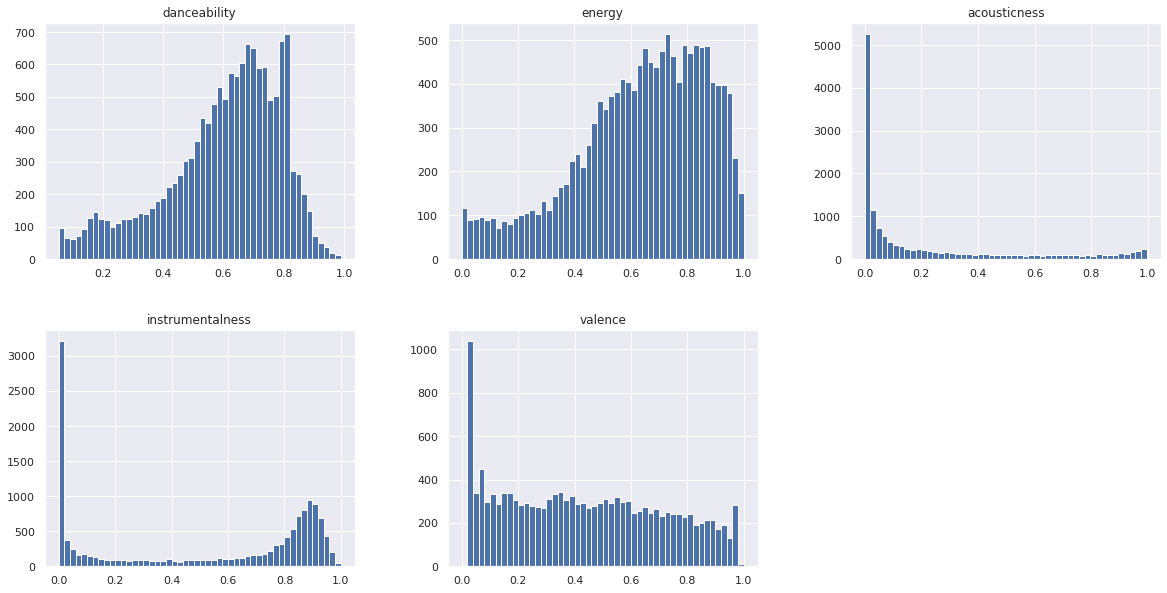
\includegraphics[width=\textwidth]{images/features-distribution.png}
      \caption{Distribution of audio features}
      \label{fig:audio_features_distribution}
\end{figure}

We can compare our single-user data with a bigger audio features dataset https://www.kaggle.com/datasets/tomigelo/spotify-audio-features.
This dataset shows similar data distributions.

I have posted a question on the Spotify Developer forum, relative to the release of a dataset
https://community.spotify.com/t5/Spotify-for-Developers/May-I-publish-an-open-source-dataset-that-contains-Spotify-Audio/td-p/5529259



\subsection{Formatting Input Data for Predicting From Last.fm Tags}

The input data passed to the XGBoost regressor is formatted in tabular format, as follows:

\begin{itemize}
      \item Given that $Tags_{k}$ is the set of most $k$ frequent Last.fm tags in the user listening history
            and, where each $tag \in Tags_{k}$.
      \item Given that $Audio$ is the set of Spotify audio features, where each $feat \in Audio$.
      \item For each $track$:
      \begin{itemize}
            \item $X_{track},_{tag}$ is the strengh of $tag$ for $track$. This value is in the $0-100$ range.
            \item $y_{track},_{feature}$ is the value of the audio feature $y$ for $track$.
      \end{itemize}
\end{itemize}

An example of this data format is provided in table \ref{tabular_tags_format}.

\begin{table}[h]
      \begin{center}
      \begin{minipage}{\textwidth}
      \caption{Tabular data format for Last.fm tags in XGBoost and Bayesian regressors}\label{tabular_tags_format}%
      \begin{tabular}{@{}lllllll@{}}
      \toprule
      Track                         & $X_{electronic}$ & $X_{ambient}$ & $X_{\dots}$ & $y_{energy}$ & $y_{valence}$ & $y_{\dots}$ \\
      \midrule
      Massive Attack - Blue Lines   & 62               & 6             &  \dots      & 0.496        & 0.947         & \dots  \\
      The Beta Band - Squares       & 40               & 3             &  \dots      & 0.446        & 0.507         & \dots  \\
      \dots                         & \dots            & \dots         &  \dots      & \dots        & \dots         & \dots  \\
      \botrule
      \end{tabular}
      \end{minipage}
      \end{center}
\end{table}

\subsection{Formatting Input Data for Predicting From Tokens}

In this particular case, the $X$ values of the tabular input data are tokens.
These tokens are obtained from passing the a string of concatenated Last.fm tags through a tokenizer.
The formal definition of this data format is as follows:

\begin{itemize}
      \item Given that $X_l$ is the token vocabulary, where $l$ is the maximum vocabulary length.
      \item Given that $Audio$ is the set of Spotify audio features, where each $feat \in Audio$.
      \item For each $track$:
      \begin{itemize}
            \item $X_{track},_{n}$ is token found at position $n$, after tokenizing the tags string.
            \item $y_{track},_{feature}$ is the value of the audio feature $y$ for $track$.
      \end{itemize}
\end{itemize}

An example of this data format is provided in table \ref{tabular_token_format}.

\begin{table}[h]
      \begin{center}
      \begin{minipage}{\textwidth}
      \caption{Tabular data format for tokens in XGBoost and Bayesian regressors}\label{tabular_token_format}%
      \begin{tabular}{@{}llllllll@{}}
      \toprule
      Track                         & $X_{0}$ & $X_{1}$ & $X_{2}$ & $X_{\dots}$ & $y_{energy}$ & $y_{valence}$ & $y_{\dots}$ \\
      \midrule
      Massive Attack - Blue Lines   & 101     & 5099    & 6154    &  \dots      & 0.496        & 0.947         &  \dots  \\
      The Beta Band - Squares       & 101     & 4522    & 2600    &  \dots      & 0.446        & 0.507         &  \dots  \\
      \dots                         & \dots   & \dots   & \dots   &  \dots      & \dots        & \dots         &  \dots  \\
      \botrule
      \end{tabular}
      \end{minipage}
      \end{center}
\end{table}


\subsection{Formatting Input Data for Predicting From Text}

When using transformer models, the input data is a string.
We must represent the Last.fm tags, which are initially in the $(tag name, tag popularity)$ form, to a a string.

After converting to a string, the formal definition of the input data is as follows:

\begin{itemize}
      \item Given that $X$ is tags represented as text.
      \item Given that $Audio$ is the set of Spotify audio features, where each $feat \in Audio$.
      \item For each $track$:
      \begin{itemize}
            \item $X_{track},_{n}$ is set of tags for $track$, encoded as a single string.
            \item $y_{track},_{feature}$ is the value of the audio feature $y$ for $track$.
      \end{itemize}
\end{itemize}

An example of this data format is provided in table \ref{text_format}.

\begin{table}[h]
      \begin{center}
      \begin{minipage}{\textwidth}
      \caption{Text data format for tokens in XGBoost and Bayesian regressors}\label{text_format}%
      \begin{tabular}{@{}lllll@{}}
      \toprule
      Track                         & $X$                                   & $y_{energy}$ & $y_{valence}$ & $y_{\dots}$ \\
      \midrule
      Massive Attack - Blue Lines   & "hip hop, chill, bristol, \dots"      & 0.496        & 0.947         & \dots  \\
      The Beta Band - Squares       & "alternative rock, folk, \dots"       & 0.446        & 0.507         & \dots \\
      \dots                         & \dots                                 & \dots        & \dots         & \dots  \\
      \botrule
      \end{tabular}
      \end{minipage}
      \end{center}
\end{table}


















\section{Experiments}

We trained a commonly used machine learning models to predict an audio feature, given the set of tags for a particular track.

\begin{itemize}
      \item Boosted tree regressor \cite{xgboost}
      \item Naive Bayes Regressor \cite{bayesian}
      \item Fine-tuned GPT-2 model
\end{itemize}

\subsection{Boosted Tree Regressor}

We configured the boosted tree regressor model with the training parameters listed in table \ref{table_xgboost_training_params}.

\begin{table}[h]
      \begin{center}
      \begin{minipage}{174pt}
      \caption{Training parameters for XGBoost regressor}\label{table_xgboost_training_params}%
      \begin{tabular}{@{}llll@{}}
      \toprule
      Parameter               & Value \\
      \midrule
      objective               & reg:squarederror  \\
      base score              & 0.5 \\
      booster                 & gbtree  \\
      colsample bylevel       & 1 \\
      colsample bynode        & 1 \\
      colsample bytree        & 1 \\
      gamma\footnotemark[1]   & 0 \\
      learning rate           & 0.300000012 \\
      max delta step          & 0 \\
      max depth               & 6 \\
      min child weight        & 1 \\
      estimators              & 200  \\
      n jobs                  & 12  \\
      num parallel tree       & 1 \\
      predictor               & auto  \\
      random state            & 0 \\
      reg alpha               & 0 \\
      reg lambda              & 1 \\
      scale pos weight        & 1 \\
      subsample               & 2 \\
      tree method             & auto  \\
      \botrule
      \end{tabular}
      \footnotetext[1]{Minimum loss reduction required to make a further partition on a leaf node of the tree.}
      \end{minipage}
      \end{center}
\end{table}


\subsection{Naive Bayes Regressor}

The Naive Bayes Regressor, and in particular, Bayesian Ridge, is the model used for regression in this case.

% COMMENT copied FROM BayesianRidge source code
% https://github.com/scikit-learn/scikit-learn/blob/9aaed4987/sklearn/linear_model/_bayes.py#L24
%
%     There exist several strategies to perform Bayesian ridge regression. This
%     implementation is based on the algorithm described in Appendix A of
%     (Tipping, 2001) where updates of the regularization parameters are done as
%     suggested in (MacKay, 1992). Note that according to A New
%     View of Automatic Relevance Determination (Wipf and Nagarajan, 2008) these
%     update rules do not guarantee that the marginal likelihood is increasing
%     between two consecutive iterations of the optimization.

The training parameters are listed in table \ref{table_bayesian_training_params}.

\begin{table}[h]
      \begin{center}
      \begin{minipage}{174pt}
      \caption{Training parameters for XGBoost regressor}\label{table_bayesian_training_params}%
      \begin{tabular}{@{}llll@{}}
      \toprule
      Parameter                     & Value \\
      \midrule
      Maximum iterations            & 300   \\
      Tolerance\footnotemark[1]     & \num{1e-03} \\
      alpha 1                       & \num{1e-06} \\
      alpha 2                       & \num{1e-06} \\
      lambda 1                      & \num{1e-06} \\
      lambda 2                      & \num{1e-06} \\
      \botrule
      \end{tabular}
      \footnotetext[1]{Tolerance for the stopping criteria.}
      \end{minipage}
      \end{center}
\end{table}


\subsection{Fine-tuned Transformer}


\textcolor{red}{TODO}

\subsection{Experiments Execution and Results}

The experiments:


\begin{table}[h]
      \begin{center}
      \begin{minipage}{\textwidth}
      \caption{Experiment results. Cells values correspond to the RMSE value.}\label{experiment_results}%
      \begin{tabular}{@{}llllll@{}}
      \toprule
      Experiment                           & Danceability    & Acousticness    & Energy    & Valence    & Instrumentalness \\
      \midrule
      $Base_token_{weight}$
      $XGBoost_Tags_{energy}$                        & 300   \\
      XGBoost - $y_{energy}$           & 300   \\
      XGBoost - Tokens - Weight Repeat     & 300   \\
      \botrule
      \end{tabular}
      \footnotetext[1]{Tolerance for the stopping criteria.}
      \end{minipage}
      \end{center}
\end{table}

\subsubsection{Results for Tabular Data Models}

\begin{figure}[h!]
      \centering
      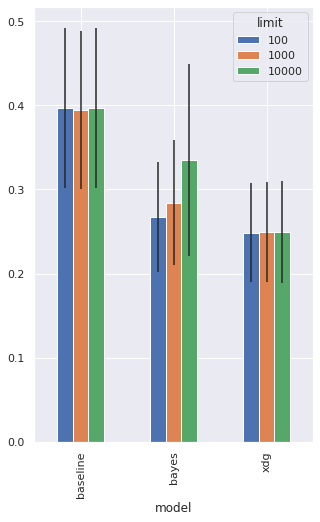
\includegraphics[width=0.5\textwidth]{images/rmse_by_model_and_limit.png}
      \caption{RMSE mean and standard deviation by model and tags/tokens limit.}
      \label{fig:rmse_by_model_and_limit}
\end{figure}


\begin{figure}[h!]
      \centering
      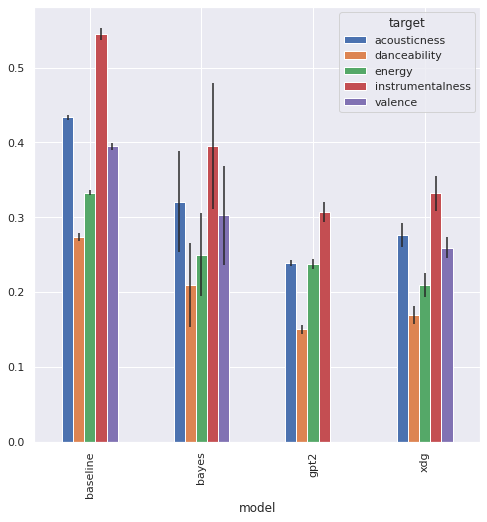
\includegraphics[width=0.7\textwidth]{images/rmse_by_model_and_feature.png}
      \caption{RMSE mean and standard deviation by model and audio feature.}
      \label{fig:rmse_by_model_and_feature}
\end{figure}


\begin{figure}[h!]
      \centering
      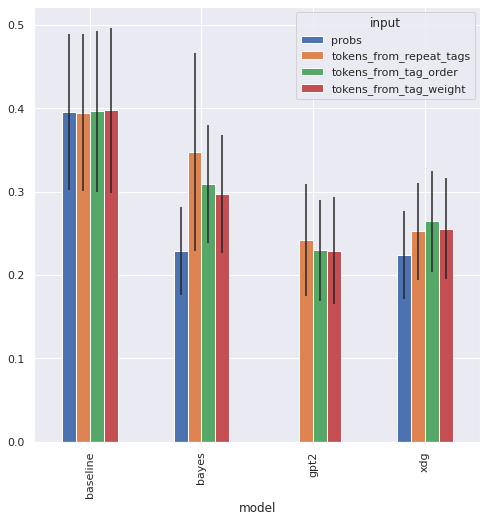
\includegraphics[width=0.7\textwidth]{images/rmse_by_model_and_input.png}
      \caption{RMSE mean and standard deviation by model and input type (tag probablities or tokens).}
      \label{fig:rmse_by_model_and_input}
\end{figure}


\begin{figure}[h!]
      \centering
      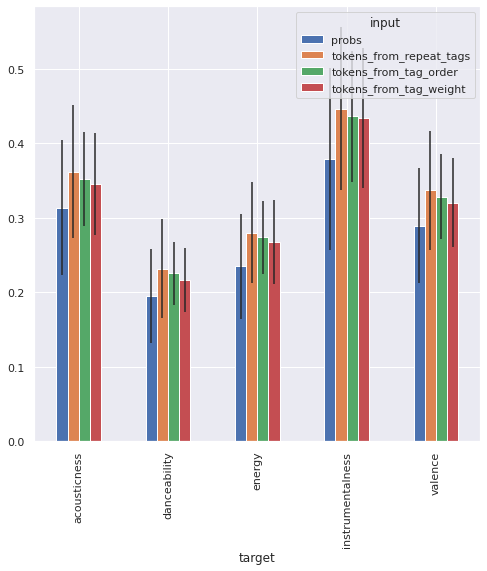
\includegraphics[width=0.7\textwidth]{images/rmse_by_feature_and_input.png}
      \caption{RMSE mean and standard deviation by audio feature and input type (tag probablities or tokens).}
      \label{fig:rmse_by_feature_and_input}
\end{figure}

\section{Conclusions}

\textcolor{red}{TODO}


\section{Acknowledgments}

\textcolor{red}{TODO}



%%===========================================================================================%%
%% If you are submitting to one of the Nature Portfolio journals, using the eJP submission   %%
%% system, please include the references within the manuscript file itself. You may do this  %%
%% by copying the reference list from your .bbl file, paste it into the main manuscript .tex %%
%% file, and delete the associated \verb+\bibliography+ commands.                            %%
%%===========================================================================================%%

\bibliography{bibliography}% common bib file
%% if required, the content of .bbl file can be included here once bbl is generated
%%\input sn-article.bbl

%% Default %%
%%\input sn-sample-bib.tex%

\end{document}
